% Created by tikzDevice version 0.12.6 on 2025-02-12 06:44:55
% !TEX encoding = UTF-8 Unicode
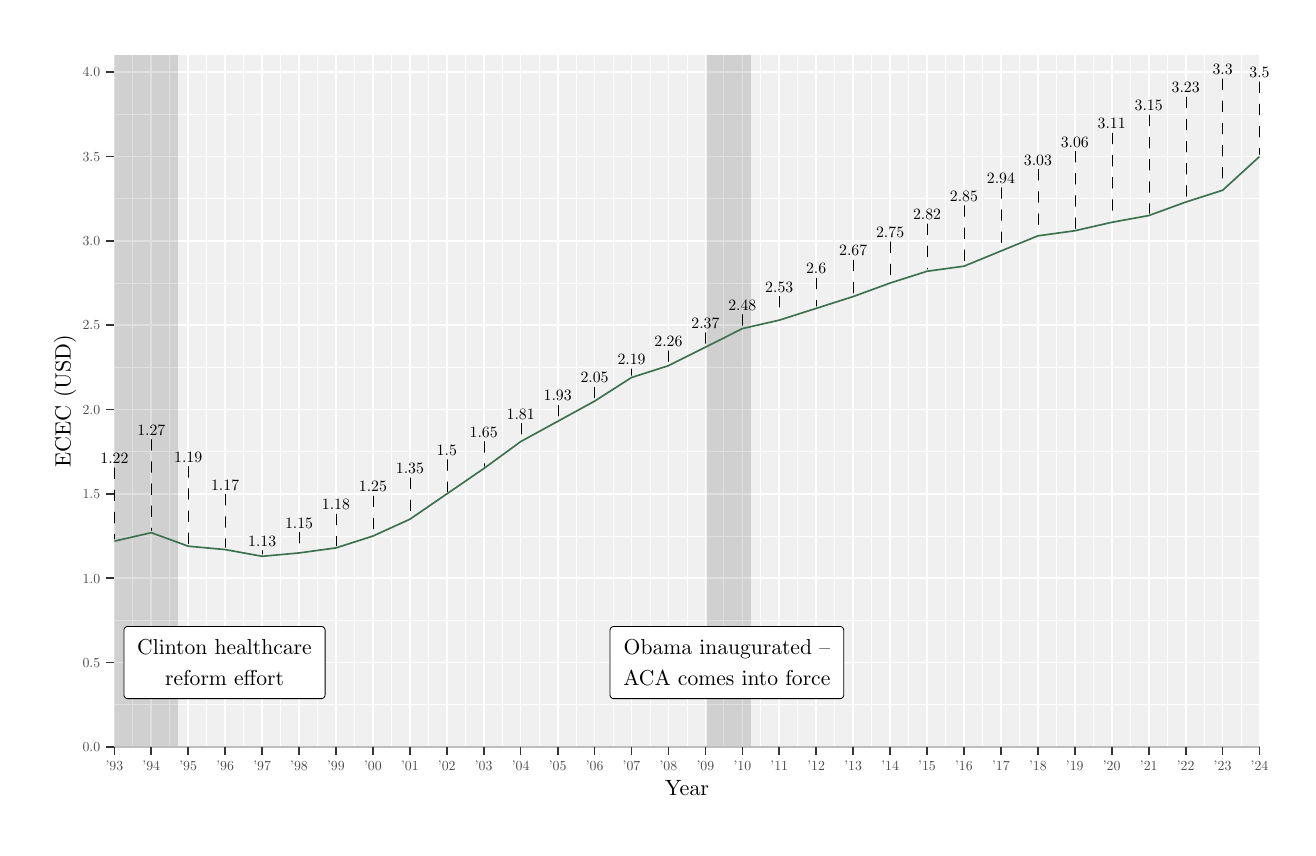
\begin{tikzpicture}[x=1pt,y=1pt]
\definecolor{fillColor}{RGB}{255,255,255}
\path[use as bounding box,fill=fillColor,fill opacity=0.00] (0,0) rectangle (455.30,289.08);
\begin{scope}
\path[clip] (  0.00,  0.00) rectangle (455.30,289.08);
\definecolor{drawColor}{RGB}{255,255,255}
\definecolor{fillColor}{RGB}{255,255,255}

\path[draw=drawColor,line width= 0.6pt,line join=round,line cap=round,fill=fillColor] (  0.00,  0.00) rectangle (455.30,289.08);
\end{scope}
\begin{scope}
\path[clip] (  0.00,  0.00) rectangle (455.30,289.08);
\definecolor{fillColor}{gray}{0.94}

\path[fill=fillColor] ( 31.15, 29.18) rectangle (445.30,279.08);
\definecolor{drawColor}{RGB}{255,255,255}

\path[draw=drawColor,line width= 0.3pt,line join=round] ( 31.15, 44.42) --
	(445.30, 44.42);

\path[draw=drawColor,line width= 0.3pt,line join=round] ( 31.15, 74.89) --
	(445.30, 74.89);

\path[draw=drawColor,line width= 0.3pt,line join=round] ( 31.15,105.37) --
	(445.30,105.37);

\path[draw=drawColor,line width= 0.3pt,line join=round] ( 31.15,135.84) --
	(445.30,135.84);

\path[draw=drawColor,line width= 0.3pt,line join=round] ( 31.15,166.32) --
	(445.30,166.32);

\path[draw=drawColor,line width= 0.3pt,line join=round] ( 31.15,196.80) --
	(445.30,196.80);

\path[draw=drawColor,line width= 0.3pt,line join=round] ( 31.15,227.27) --
	(445.30,227.27);

\path[draw=drawColor,line width= 0.3pt,line join=round] ( 31.15,257.75) --
	(445.30,257.75);

\path[draw=drawColor,line width= 0.3pt,line join=round] ( 38.00, 29.18) --
	( 38.00,279.08);

\path[draw=drawColor,line width= 0.3pt,line join=round] ( 51.34, 29.18) --
	( 51.34,279.08);

\path[draw=drawColor,line width= 0.3pt,line join=round] ( 64.68, 29.18) --
	( 64.68,279.08);

\path[draw=drawColor,line width= 0.3pt,line join=round] ( 78.04, 29.18) --
	( 78.04,279.08);

\path[draw=drawColor,line width= 0.3pt,line join=round] ( 91.40, 29.18) --
	( 91.40,279.08);

\path[draw=drawColor,line width= 0.3pt,line join=round] (104.74, 29.18) --
	(104.74,279.08);

\path[draw=drawColor,line width= 0.3pt,line join=round] (118.08, 29.18) --
	(118.08,279.08);

\path[draw=drawColor,line width= 0.3pt,line join=round] (131.44, 29.18) --
	(131.44,279.08);

\path[draw=drawColor,line width= 0.3pt,line join=round] (144.79, 29.18) --
	(144.79,279.08);

\path[draw=drawColor,line width= 0.3pt,line join=round] (158.13, 29.18) --
	(158.13,279.08);

\path[draw=drawColor,line width= 0.3pt,line join=round] (171.47, 29.18) --
	(171.47,279.08);

\path[draw=drawColor,line width= 0.3pt,line join=round] (184.83, 29.18) --
	(184.83,279.08);

\path[draw=drawColor,line width= 0.3pt,line join=round] (198.19, 29.18) --
	(198.19,279.08);

\path[draw=drawColor,line width= 0.3pt,line join=round] (211.53, 29.18) --
	(211.53,279.08);

\path[draw=drawColor,line width= 0.3pt,line join=round] (224.87, 29.18) --
	(224.87,279.08);

\path[draw=drawColor,line width= 0.3pt,line join=round] (238.23, 29.18) --
	(238.23,279.08);

\path[draw=drawColor,line width= 0.3pt,line join=round] (251.58, 29.18) --
	(251.58,279.08);

\path[draw=drawColor,line width= 0.3pt,line join=round] (264.92, 29.18) --
	(264.92,279.08);

\path[draw=drawColor,line width= 0.3pt,line join=round] (278.26, 29.18) --
	(278.26,279.08);

\path[draw=drawColor,line width= 0.3pt,line join=round] (291.62, 29.18) --
	(291.62,279.08);

\path[draw=drawColor,line width= 0.3pt,line join=round] (304.98, 29.18) --
	(304.98,279.08);

\path[draw=drawColor,line width= 0.3pt,line join=round] (318.32, 29.18) --
	(318.32,279.08);

\path[draw=drawColor,line width= 0.3pt,line join=round] (331.66, 29.18) --
	(331.66,279.08);

\path[draw=drawColor,line width= 0.3pt,line join=round] (345.02, 29.18) --
	(345.02,279.08);

\path[draw=drawColor,line width= 0.3pt,line join=round] (358.37, 29.18) --
	(358.37,279.08);

\path[draw=drawColor,line width= 0.3pt,line join=round] (371.71, 29.18) --
	(371.71,279.08);

\path[draw=drawColor,line width= 0.3pt,line join=round] (385.05, 29.18) --
	(385.05,279.08);

\path[draw=drawColor,line width= 0.3pt,line join=round] (398.41, 29.18) --
	(398.41,279.08);

\path[draw=drawColor,line width= 0.3pt,line join=round] (411.77, 29.18) --
	(411.77,279.08);

\path[draw=drawColor,line width= 0.3pt,line join=round] (425.11, 29.18) --
	(425.11,279.08);

\path[draw=drawColor,line width= 0.3pt,line join=round] (438.45, 29.18) --
	(438.45,279.08);

\path[draw=drawColor,line width= 0.6pt,line join=round] ( 31.15, 29.18) --
	(445.30, 29.18);

\path[draw=drawColor,line width= 0.6pt,line join=round] ( 31.15, 59.66) --
	(445.30, 59.66);

\path[draw=drawColor,line width= 0.6pt,line join=round] ( 31.15, 90.13) --
	(445.30, 90.13);

\path[draw=drawColor,line width= 0.6pt,line join=round] ( 31.15,120.61) --
	(445.30,120.61);

\path[draw=drawColor,line width= 0.6pt,line join=round] ( 31.15,151.08) --
	(445.30,151.08);

\path[draw=drawColor,line width= 0.6pt,line join=round] ( 31.15,181.56) --
	(445.30,181.56);

\path[draw=drawColor,line width= 0.6pt,line join=round] ( 31.15,212.03) --
	(445.30,212.03);

\path[draw=drawColor,line width= 0.6pt,line join=round] ( 31.15,242.51) --
	(445.30,242.51);

\path[draw=drawColor,line width= 0.6pt,line join=round] ( 31.15,272.98) --
	(445.30,272.98);

\path[draw=drawColor,line width= 0.6pt,line join=round] ( 31.34, 29.18) --
	( 31.34,279.08);

\path[draw=drawColor,line width= 0.6pt,line join=round] ( 44.67, 29.18) --
	( 44.67,279.08);

\path[draw=drawColor,line width= 0.6pt,line join=round] ( 58.01, 29.18) --
	( 58.01,279.08);

\path[draw=drawColor,line width= 0.6pt,line join=round] ( 71.35, 29.18) --
	( 71.35,279.08);

\path[draw=drawColor,line width= 0.6pt,line join=round] ( 84.73, 29.18) --
	( 84.73,279.08);

\path[draw=drawColor,line width= 0.6pt,line join=round] ( 98.07, 29.18) --
	( 98.07,279.08);

\path[draw=drawColor,line width= 0.6pt,line join=round] (111.41, 29.18) --
	(111.41,279.08);

\path[draw=drawColor,line width= 0.6pt,line join=round] (124.75, 29.18) --
	(124.75,279.08);

\path[draw=drawColor,line width= 0.6pt,line join=round] (138.12, 29.18) --
	(138.12,279.08);

\path[draw=drawColor,line width= 0.6pt,line join=round] (151.46, 29.18) --
	(151.46,279.08);

\path[draw=drawColor,line width= 0.6pt,line join=round] (164.80, 29.18) --
	(164.80,279.08);

\path[draw=drawColor,line width= 0.6pt,line join=round] (178.14, 29.18) --
	(178.14,279.08);

\path[draw=drawColor,line width= 0.6pt,line join=round] (191.52, 29.18) --
	(191.52,279.08);

\path[draw=drawColor,line width= 0.6pt,line join=round] (204.86, 29.18) --
	(204.86,279.08);

\path[draw=drawColor,line width= 0.6pt,line join=round] (218.20, 29.18) --
	(218.20,279.08);

\path[draw=drawColor,line width= 0.6pt,line join=round] (231.54, 29.18) --
	(231.54,279.08);

\path[draw=drawColor,line width= 0.6pt,line join=round] (244.91, 29.18) --
	(244.91,279.08);

\path[draw=drawColor,line width= 0.6pt,line join=round] (258.25, 29.18) --
	(258.25,279.08);

\path[draw=drawColor,line width= 0.6pt,line join=round] (271.59, 29.18) --
	(271.59,279.08);

\path[draw=drawColor,line width= 0.6pt,line join=round] (284.93, 29.18) --
	(284.93,279.08);

\path[draw=drawColor,line width= 0.6pt,line join=round] (298.31, 29.18) --
	(298.31,279.08);

\path[draw=drawColor,line width= 0.6pt,line join=round] (311.65, 29.18) --
	(311.65,279.08);

\path[draw=drawColor,line width= 0.6pt,line join=round] (324.99, 29.18) --
	(324.99,279.08);

\path[draw=drawColor,line width= 0.6pt,line join=round] (338.33, 29.18) --
	(338.33,279.08);

\path[draw=drawColor,line width= 0.6pt,line join=round] (351.70, 29.18) --
	(351.70,279.08);

\path[draw=drawColor,line width= 0.6pt,line join=round] (365.04, 29.18) --
	(365.04,279.08);

\path[draw=drawColor,line width= 0.6pt,line join=round] (378.38, 29.18) --
	(378.38,279.08);

\path[draw=drawColor,line width= 0.6pt,line join=round] (391.72, 29.18) --
	(391.72,279.08);

\path[draw=drawColor,line width= 0.6pt,line join=round] (405.10, 29.18) --
	(405.10,279.08);

\path[draw=drawColor,line width= 0.6pt,line join=round] (418.44, 29.18) --
	(418.44,279.08);

\path[draw=drawColor,line width= 0.6pt,line join=round] (431.78, 29.18) --
	(431.78,279.08);

\path[draw=drawColor,line width= 0.6pt,line join=round] (445.12, 29.18) --
	(445.12,279.08);
\definecolor{fillColor}{RGB}{190,190,190}

\path[fill=fillColor,fill opacity=0.01] ( 31.34, 29.18) rectangle ( 54.47,279.08);

\path[fill=fillColor,fill opacity=0.01] ( 31.34, 29.18) rectangle ( 54.47,279.08);

\path[fill=fillColor,fill opacity=0.01] ( 31.34, 29.18) rectangle ( 54.47,279.08);

\path[fill=fillColor,fill opacity=0.01] ( 31.34, 29.18) rectangle ( 54.47,279.08);

\path[fill=fillColor,fill opacity=0.01] ( 31.34, 29.18) rectangle ( 54.47,279.08);

\path[fill=fillColor,fill opacity=0.01] ( 31.34, 29.18) rectangle ( 54.47,279.08);

\path[fill=fillColor,fill opacity=0.01] ( 31.34, 29.18) rectangle ( 54.47,279.08);

\path[fill=fillColor,fill opacity=0.01] ( 31.34, 29.18) rectangle ( 54.47,279.08);

\path[fill=fillColor,fill opacity=0.01] ( 31.34, 29.18) rectangle ( 54.47,279.08);

\path[fill=fillColor,fill opacity=0.01] ( 31.34, 29.18) rectangle ( 54.47,279.08);

\path[fill=fillColor,fill opacity=0.01] ( 31.34, 29.18) rectangle ( 54.47,279.08);

\path[fill=fillColor,fill opacity=0.01] ( 31.34, 29.18) rectangle ( 54.47,279.08);

\path[fill=fillColor,fill opacity=0.01] ( 31.34, 29.18) rectangle ( 54.47,279.08);

\path[fill=fillColor,fill opacity=0.01] ( 31.34, 29.18) rectangle ( 54.47,279.08);

\path[fill=fillColor,fill opacity=0.01] ( 31.34, 29.18) rectangle ( 54.47,279.08);

\path[fill=fillColor,fill opacity=0.01] ( 31.34, 29.18) rectangle ( 54.47,279.08);

\path[fill=fillColor,fill opacity=0.01] ( 31.34, 29.18) rectangle ( 54.47,279.08);

\path[fill=fillColor,fill opacity=0.01] ( 31.34, 29.18) rectangle ( 54.47,279.08);

\path[fill=fillColor,fill opacity=0.01] ( 31.34, 29.18) rectangle ( 54.47,279.08);

\path[fill=fillColor,fill opacity=0.01] ( 31.34, 29.18) rectangle ( 54.47,279.08);

\path[fill=fillColor,fill opacity=0.01] ( 31.34, 29.18) rectangle ( 54.47,279.08);

\path[fill=fillColor,fill opacity=0.01] ( 31.34, 29.18) rectangle ( 54.47,279.08);

\path[fill=fillColor,fill opacity=0.01] ( 31.34, 29.18) rectangle ( 54.47,279.08);

\path[fill=fillColor,fill opacity=0.01] ( 31.34, 29.18) rectangle ( 54.47,279.08);

\path[fill=fillColor,fill opacity=0.01] ( 31.34, 29.18) rectangle ( 54.47,279.08);

\path[fill=fillColor,fill opacity=0.01] ( 31.34, 29.18) rectangle ( 54.47,279.08);

\path[fill=fillColor,fill opacity=0.01] ( 31.34, 29.18) rectangle ( 54.47,279.08);

\path[fill=fillColor,fill opacity=0.01] ( 31.34, 29.18) rectangle ( 54.47,279.08);

\path[fill=fillColor,fill opacity=0.01] ( 31.34, 29.18) rectangle ( 54.47,279.08);

\path[fill=fillColor,fill opacity=0.01] ( 31.34, 29.18) rectangle ( 54.47,279.08);

\path[fill=fillColor,fill opacity=0.01] ( 31.34, 29.18) rectangle ( 54.47,279.08);

\path[fill=fillColor,fill opacity=0.01] ( 31.34, 29.18) rectangle ( 54.47,279.08);

\path[fill=fillColor,fill opacity=0.01] (245.61, 29.18) rectangle (261.21,279.08);

\path[fill=fillColor,fill opacity=0.01] (245.61, 29.18) rectangle (261.21,279.08);

\path[fill=fillColor,fill opacity=0.01] (245.61, 29.18) rectangle (261.21,279.08);

\path[fill=fillColor,fill opacity=0.01] (245.61, 29.18) rectangle (261.21,279.08);

\path[fill=fillColor,fill opacity=0.01] (245.61, 29.18) rectangle (261.21,279.08);

\path[fill=fillColor,fill opacity=0.01] (245.61, 29.18) rectangle (261.21,279.08);

\path[fill=fillColor,fill opacity=0.01] (245.61, 29.18) rectangle (261.21,279.08);

\path[fill=fillColor,fill opacity=0.01] (245.61, 29.18) rectangle (261.21,279.08);

\path[fill=fillColor,fill opacity=0.01] (245.61, 29.18) rectangle (261.21,279.08);

\path[fill=fillColor,fill opacity=0.01] (245.61, 29.18) rectangle (261.21,279.08);

\path[fill=fillColor,fill opacity=0.01] (245.61, 29.18) rectangle (261.21,279.08);

\path[fill=fillColor,fill opacity=0.01] (245.61, 29.18) rectangle (261.21,279.08);

\path[fill=fillColor,fill opacity=0.01] (245.61, 29.18) rectangle (261.21,279.08);

\path[fill=fillColor,fill opacity=0.01] (245.61, 29.18) rectangle (261.21,279.08);

\path[fill=fillColor,fill opacity=0.01] (245.61, 29.18) rectangle (261.21,279.08);

\path[fill=fillColor,fill opacity=0.01] (245.61, 29.18) rectangle (261.21,279.08);

\path[fill=fillColor,fill opacity=0.01] (245.61, 29.18) rectangle (261.21,279.08);

\path[fill=fillColor,fill opacity=0.01] (245.61, 29.18) rectangle (261.21,279.08);

\path[fill=fillColor,fill opacity=0.01] (245.61, 29.18) rectangle (261.21,279.08);

\path[fill=fillColor,fill opacity=0.01] (245.61, 29.18) rectangle (261.21,279.08);

\path[fill=fillColor,fill opacity=0.01] (245.61, 29.18) rectangle (261.21,279.08);

\path[fill=fillColor,fill opacity=0.01] (245.61, 29.18) rectangle (261.21,279.08);

\path[fill=fillColor,fill opacity=0.01] (245.61, 29.18) rectangle (261.21,279.08);

\path[fill=fillColor,fill opacity=0.01] (245.61, 29.18) rectangle (261.21,279.08);

\path[fill=fillColor,fill opacity=0.01] (245.61, 29.18) rectangle (261.21,279.08);

\path[fill=fillColor,fill opacity=0.01] (245.61, 29.18) rectangle (261.21,279.08);

\path[fill=fillColor,fill opacity=0.01] (245.61, 29.18) rectangle (261.21,279.08);

\path[fill=fillColor,fill opacity=0.01] (245.61, 29.18) rectangle (261.21,279.08);

\path[fill=fillColor,fill opacity=0.01] (245.61, 29.18) rectangle (261.21,279.08);

\path[fill=fillColor,fill opacity=0.01] (245.61, 29.18) rectangle (261.21,279.08);

\path[fill=fillColor,fill opacity=0.01] (245.61, 29.18) rectangle (261.21,279.08);

\path[fill=fillColor,fill opacity=0.01] (245.61, 29.18) rectangle (261.21,279.08);
\definecolor{drawColor}{RGB}{190,190,190}

\path[draw=drawColor,line width= 0.6pt,line join=round] ( 31.15, 29.18) -- (445.30, 29.18);
\definecolor{drawColor}{RGB}{60,113,79}

\path[draw=drawColor,line width= 0.6pt,line join=round] ( 31.34,103.54) --
	( 44.67,106.59) --
	( 58.01,101.71) --
	( 71.35,100.49) --
	( 84.73, 98.06) --
	( 98.07, 99.27) --
	(111.41,101.10) --
	(124.75,105.37) --
	(138.12,111.46) --
	(151.46,120.61) --
	(164.80,129.75) --
	(178.14,139.50) --
	(191.52,146.82) --
	(204.86,154.13) --
	(218.20,162.66) --
	(231.54,166.93) --
	(244.91,173.63) --
	(258.25,180.34) --
	(271.59,183.39) --
	(284.93,187.65) --
	(298.31,191.92) --
	(311.65,196.80) --
	(324.99,201.06) --
	(338.33,202.89) --
	(351.70,208.38) --
	(365.04,213.86) --
	(378.38,215.69) --
	(391.72,218.74) --
	(405.10,221.18) --
	(418.44,226.05) --
	(431.78,230.32) --
	(445.12,242.51);
\definecolor{drawColor}{RGB}{0,0,0}

\path[draw=drawColor,line width= 0.1pt,dash pattern=on 4pt off 4pt ,line join=round,line cap=round] ( 31.34,130.08) -- ( 31.34,104.27);

\path[draw=drawColor,line width= 0.1pt,dash pattern=on 4pt off 4pt ,line join=round,line cap=round] ( 44.67,140.32) -- ( 44.67,107.32);

\path[draw=drawColor,line width= 0.1pt,dash pattern=on 4pt off 4pt ,line join=round,line cap=round] ( 58.01,130.55) -- ( 58.01,102.44);

\path[draw=drawColor,line width= 0.1pt,dash pattern=on 4pt off 4pt ,line join=round,line cap=round] ( 71.35,120.47) -- ( 71.35,101.22);

\path[draw=drawColor,line width= 0.1pt,dash pattern=on 4pt off 4pt ,line join=round,line cap=round] ( 84.73,100.20) -- ( 84.73, 98.78);

\path[draw=drawColor,line width= 0.1pt,dash pattern=on 4pt off 4pt ,line join=round,line cap=round] ( 98.07,106.77) -- ( 98.07,100.00);

\path[draw=drawColor,line width= 0.1pt,dash pattern=on 4pt off 4pt ,line join=round,line cap=round] (111.41,113.34) -- (111.41,101.83);

\path[draw=drawColor,line width= 0.1pt,dash pattern=on 4pt off 4pt ,line join=round,line cap=round] (124.75,119.91) -- (124.75,106.10);

\path[draw=drawColor,line width= 0.1pt,dash pattern=on 4pt off 4pt ,line join=round,line cap=round] (138.12,126.45) -- (138.12,112.19);

\path[draw=drawColor,line width= 0.1pt,dash pattern=on 4pt off 4pt ,line join=round,line cap=round] (151.46,133.02) -- (151.46,121.34);

\path[draw=drawColor,line width= 0.1pt,dash pattern=on 4pt off 4pt ,line join=round,line cap=round] (164.80,139.59) -- (164.80,130.48);

\path[draw=drawColor,line width= 0.1pt,dash pattern=on 4pt off 4pt ,line join=round,line cap=round] (178.14,146.15) -- (178.14,140.23);

\path[draw=drawColor,line width= 0.1pt,dash pattern=on 4pt off 4pt ,line join=round,line cap=round] (191.52,152.69) -- (191.52,147.54);

\path[draw=drawColor,line width= 0.1pt,dash pattern=on 4pt off 4pt ,line join=round,line cap=round] (204.86,159.26) -- (204.86,154.86);

\path[draw=drawColor,line width= 0.1pt,dash pattern=on 4pt off 4pt ,line join=round,line cap=round] (218.20,165.82) -- (218.20,163.39);

\path[draw=drawColor,line width= 0.1pt,dash pattern=on 4pt off 4pt ,line join=round,line cap=round] (231.54,172.39) -- (231.54,167.66);

\path[draw=drawColor,line width= 0.1pt,dash pattern=on 4pt off 4pt ,line join=round,line cap=round] (244.91,178.92) -- (244.91,174.36);

\path[draw=drawColor,line width= 0.1pt,dash pattern=on 4pt off 4pt ,line join=round,line cap=round] (258.25,185.48) -- (258.25,181.07);

\path[draw=drawColor,line width= 0.1pt,dash pattern=on 4pt off 4pt ,line join=round,line cap=round] (271.59,192.05) -- (271.59,184.12);

\path[draw=drawColor,line width= 0.1pt,dash pattern=on 4pt off 4pt ,line join=round,line cap=round] (284.93,198.61) -- (284.93,188.38);

\path[draw=drawColor,line width= 0.1pt,dash pattern=on 4pt off 4pt ,line join=round,line cap=round] (298.31,205.14) -- (298.31,192.65);

\path[draw=drawColor,line width= 0.1pt,dash pattern=on 4pt off 4pt ,line join=round,line cap=round] (311.65,211.70) -- (311.65,197.52);

\path[draw=drawColor,line width= 0.1pt,dash pattern=on 4pt off 4pt ,line join=round,line cap=round] (324.99,218.25) -- (324.99,201.79);

\path[draw=drawColor,line width= 0.1pt,dash pattern=on 4pt off 4pt ,line join=round,line cap=round] (338.33,224.81) -- (338.33,203.62);

\path[draw=drawColor,line width= 0.1pt,dash pattern=on 4pt off 4pt ,line join=round,line cap=round] (351.70,231.34) -- (351.70,209.11);

\path[draw=drawColor,line width= 0.1pt,dash pattern=on 4pt off 4pt ,line join=round,line cap=round] (365.04,237.90) -- (365.04,214.59);

\path[draw=drawColor,line width= 0.1pt,dash pattern=on 4pt off 4pt ,line join=round,line cap=round] (378.38,244.45) -- (378.38,216.42);

\path[draw=drawColor,line width= 0.1pt,dash pattern=on 4pt off 4pt ,line join=round,line cap=round] (391.72,251.01) -- (391.72,219.47);

\path[draw=drawColor,line width= 0.1pt,dash pattern=on 4pt off 4pt ,line join=round,line cap=round] (405.10,257.53) -- (405.10,221.91);

\path[draw=drawColor,line width= 0.1pt,dash pattern=on 4pt off 4pt ,line join=round,line cap=round] (418.44,264.09) -- (418.44,226.78);

\path[draw=drawColor,line width= 0.1pt,dash pattern=on 4pt off 4pt ,line join=round,line cap=round] (431.78,270.64) -- (431.78,231.05);

\path[draw=drawColor,line width= 0.1pt,dash pattern=on 4pt off 4pt ,line join=round,line cap=round] (445.12,269.52) -- (445.12,243.24);

\node[text=drawColor,anchor=base,inner sep=0pt, outer sep=0pt, scale=  0.57] at ( 31.34,131.58) {1.22};

\node[text=drawColor,anchor=base,inner sep=0pt, outer sep=0pt, scale=  0.57] at ( 44.67,141.83) {1.27};

\node[text=drawColor,anchor=base,inner sep=0pt, outer sep=0pt, scale=  0.57] at ( 58.01,132.05) {1.19};

\node[text=drawColor,anchor=base,inner sep=0pt, outer sep=0pt, scale=  0.57] at ( 71.35,121.98) {1.17};

\node[text=drawColor,anchor=base,inner sep=0pt, outer sep=0pt, scale=  0.57] at ( 84.73,101.71) {1.13};

\node[text=drawColor,anchor=base,inner sep=0pt, outer sep=0pt, scale=  0.57] at ( 98.07,108.28) {1.15};

\node[text=drawColor,anchor=base,inner sep=0pt, outer sep=0pt, scale=  0.57] at (111.41,114.84) {1.18};

\node[text=drawColor,anchor=base,inner sep=0pt, outer sep=0pt, scale=  0.57] at (124.75,121.41) {1.25};

\node[text=drawColor,anchor=base,inner sep=0pt, outer sep=0pt, scale=  0.57] at (138.12,127.96) {1.35};

\node[text=drawColor,anchor=base,inner sep=0pt, outer sep=0pt, scale=  0.57] at (151.46,134.52) {1.5};

\node[text=drawColor,anchor=base,inner sep=0pt, outer sep=0pt, scale=  0.57] at (164.80,141.09) {1.65};

\node[text=drawColor,anchor=base,inner sep=0pt, outer sep=0pt, scale=  0.57] at (178.14,147.66) {1.81};

\node[text=drawColor,anchor=base,inner sep=0pt, outer sep=0pt, scale=  0.57] at (191.52,154.20) {1.93};

\node[text=drawColor,anchor=base,inner sep=0pt, outer sep=0pt, scale=  0.57] at (204.86,160.76) {2.05};

\node[text=drawColor,anchor=base,inner sep=0pt, outer sep=0pt, scale=  0.57] at (218.20,167.33) {2.19};

\node[text=drawColor,anchor=base,inner sep=0pt, outer sep=0pt, scale=  0.57] at (231.54,173.89) {2.26};

\node[text=drawColor,anchor=base,inner sep=0pt, outer sep=0pt, scale=  0.57] at (244.91,180.43) {2.37};

\node[text=drawColor,anchor=base,inner sep=0pt, outer sep=0pt, scale=  0.57] at (258.25,186.99) {2.48};

\node[text=drawColor,anchor=base,inner sep=0pt, outer sep=0pt, scale=  0.57] at (271.59,193.55) {2.53};

\node[text=drawColor,anchor=base,inner sep=0pt, outer sep=0pt, scale=  0.57] at (284.93,200.11) {2.6};

\node[text=drawColor,anchor=base,inner sep=0pt, outer sep=0pt, scale=  0.57] at (298.31,206.64) {2.67};

\node[text=drawColor,anchor=base,inner sep=0pt, outer sep=0pt, scale=  0.57] at (311.65,213.20) {2.75};

\node[text=drawColor,anchor=base,inner sep=0pt, outer sep=0pt, scale=  0.57] at (324.99,219.76) {2.82};

\node[text=drawColor,anchor=base,inner sep=0pt, outer sep=0pt, scale=  0.57] at (338.33,226.32) {2.85};

\node[text=drawColor,anchor=base,inner sep=0pt, outer sep=0pt, scale=  0.57] at (351.70,232.85) {2.94};

\node[text=drawColor,anchor=base,inner sep=0pt, outer sep=0pt, scale=  0.57] at (365.04,239.40) {3.03};

\node[text=drawColor,anchor=base,inner sep=0pt, outer sep=0pt, scale=  0.57] at (378.38,245.96) {3.06};

\node[text=drawColor,anchor=base,inner sep=0pt, outer sep=0pt, scale=  0.57] at (391.72,252.51) {3.11};

\node[text=drawColor,anchor=base,inner sep=0pt, outer sep=0pt, scale=  0.57] at (405.10,259.04) {3.15};

\node[text=drawColor,anchor=base,inner sep=0pt, outer sep=0pt, scale=  0.57] at (418.44,265.59) {3.23};

\node[text=drawColor,anchor=base,inner sep=0pt, outer sep=0pt, scale=  0.57] at (431.78,272.15) {3.3};

\node[text=drawColor,anchor=base,inner sep=0pt, outer sep=0pt, scale=  0.57] at (445.12,271.03) {3.5};
\definecolor{fillColor}{RGB}{255,255,255}

\path[draw=drawColor,line width= 0.3pt,line join=round,line cap=round,fill=fillColor] ( 36.21, 46.62) --
	(106.06, 46.62) --
	(106.01, 46.62) --
	(106.23, 46.63) --
	(106.46, 46.67) --
	(106.67, 46.75) --
	(106.87, 46.87) --
	(107.04, 47.01) --
	(107.19, 47.18) --
	(107.31, 47.37) --
	(107.40, 47.58) --
	(107.46, 47.80) --
	(107.48, 48.03) --
	(107.48, 48.03) --
	(107.48, 71.28) --
	(107.48, 71.28) --
	(107.46, 71.51) --
	(107.40, 71.73) --
	(107.31, 71.94) --
	(107.19, 72.13) --
	(107.04, 72.30) --
	(106.87, 72.45) --
	(106.67, 72.56) --
	(106.46, 72.64) --
	(106.23, 72.69) --
	(106.06, 72.70) --
	( 36.21, 72.70) --
	( 36.38, 72.69) --
	( 36.15, 72.70) --
	( 35.92, 72.67) --
	( 35.71, 72.60) --
	( 35.50, 72.51) --
	( 35.31, 72.38) --
	( 35.15, 72.22) --
	( 35.01, 72.04) --
	( 34.91, 71.84) --
	( 34.83, 71.62) --
	( 34.80, 71.40) --
	( 34.79, 71.28) --
	( 34.79, 48.03) --
	( 34.80, 48.14) --
	( 34.80, 47.92) --
	( 34.83, 47.69) --
	( 34.91, 47.48) --
	( 35.01, 47.27) --
	( 35.15, 47.09) --
	( 35.31, 46.93) --
	( 35.50, 46.80) --
	( 35.71, 46.71) --
	( 35.92, 46.64) --
	( 36.15, 46.62) --
	cycle;
\end{scope}
\begin{scope}
\path[clip] (  0.00,  0.00) rectangle (455.30,289.08);
\definecolor{drawColor}{RGB}{0,0,0}

\node[text=drawColor,anchor=base,inner sep=0pt, outer sep=0pt, scale=  0.78] at ( 71.13, 62.60) {Clinton healthcare };

\node[text=drawColor,anchor=base,inner sep=0pt, outer sep=0pt, scale=  0.78] at ( 71.13, 51.33) { reform effort};
\end{scope}
\begin{scope}
\path[clip] (  0.00,  0.00) rectangle (455.30,289.08);
\definecolor{drawColor}{RGB}{0,0,0}
\definecolor{fillColor}{RGB}{255,255,255}

\path[draw=drawColor,line width= 0.3pt,line join=round,line cap=round,fill=fillColor] (211.85, 46.62) --
	(293.48, 46.62) --
	(293.42, 46.62) --
	(293.65, 46.63) --
	(293.87, 46.67) --
	(294.09, 46.75) --
	(294.28, 46.87) --
	(294.46, 47.01) --
	(294.61, 47.18) --
	(294.73, 47.37) --
	(294.82, 47.58) --
	(294.87, 47.80) --
	(294.89, 48.03) --
	(294.89, 48.03) --
	(294.89, 71.28) --
	(294.89, 71.28) --
	(294.87, 71.51) --
	(294.82, 71.73) --
	(294.73, 71.94) --
	(294.61, 72.13) --
	(294.46, 72.30) --
	(294.28, 72.45) --
	(294.09, 72.56) --
	(293.87, 72.64) --
	(293.65, 72.69) --
	(293.48, 72.70) --
	(211.85, 72.70) --
	(212.02, 72.69) --
	(211.79, 72.70) --
	(211.56, 72.67) --
	(211.34, 72.60) --
	(211.14, 72.51) --
	(210.95, 72.38) --
	(210.79, 72.22) --
	(210.65, 72.04) --
	(210.55, 71.84) --
	(210.47, 71.62) --
	(210.44, 71.40) --
	(210.43, 71.28) --
	(210.43, 48.03) --
	(210.44, 48.14) --
	(210.44, 47.92) --
	(210.47, 47.69) --
	(210.55, 47.48) --
	(210.65, 47.27) --
	(210.79, 47.09) --
	(210.95, 46.93) --
	(211.14, 46.80) --
	(211.34, 46.71) --
	(211.56, 46.64) --
	(211.79, 46.62) --
	cycle;
\end{scope}
\begin{scope}
\path[clip] (  0.00,  0.00) rectangle (455.30,289.08);
\definecolor{drawColor}{RGB}{0,0,0}

\node[text=drawColor,anchor=base,inner sep=0pt, outer sep=0pt, scale=  0.78] at (252.66, 62.60) {Obama inaugurated -- };

\node[text=drawColor,anchor=base,inner sep=0pt, outer sep=0pt, scale=  0.78] at (252.66, 51.33) { ACA comes into force};
\end{scope}
\begin{scope}
\path[clip] (  0.00,  0.00) rectangle (455.30,289.08);
\definecolor{drawColor}{gray}{0.30}

\node[text=drawColor,anchor=base east,inner sep=0pt, outer sep=0pt, scale=  0.50] at ( 26.20, 27.46) {0.0};

\node[text=drawColor,anchor=base east,inner sep=0pt, outer sep=0pt, scale=  0.50] at ( 26.20, 57.93) {0.5};

\node[text=drawColor,anchor=base east,inner sep=0pt, outer sep=0pt, scale=  0.50] at ( 26.20, 88.41) {1.0};

\node[text=drawColor,anchor=base east,inner sep=0pt, outer sep=0pt, scale=  0.50] at ( 26.20,118.89) {1.5};

\node[text=drawColor,anchor=base east,inner sep=0pt, outer sep=0pt, scale=  0.50] at ( 26.20,149.36) {2.0};

\node[text=drawColor,anchor=base east,inner sep=0pt, outer sep=0pt, scale=  0.50] at ( 26.20,179.84) {2.5};

\node[text=drawColor,anchor=base east,inner sep=0pt, outer sep=0pt, scale=  0.50] at ( 26.20,210.31) {3.0};

\node[text=drawColor,anchor=base east,inner sep=0pt, outer sep=0pt, scale=  0.50] at ( 26.20,240.79) {3.5};

\node[text=drawColor,anchor=base east,inner sep=0pt, outer sep=0pt, scale=  0.50] at ( 26.20,271.26) {4.0};
\end{scope}
\begin{scope}
\path[clip] (  0.00,  0.00) rectangle (455.30,289.08);
\definecolor{drawColor}{gray}{0.20}

\path[draw=drawColor,line width= 0.6pt,line join=round] ( 28.40, 29.18) --
	( 31.15, 29.18);

\path[draw=drawColor,line width= 0.6pt,line join=round] ( 28.40, 59.66) --
	( 31.15, 59.66);

\path[draw=drawColor,line width= 0.6pt,line join=round] ( 28.40, 90.13) --
	( 31.15, 90.13);

\path[draw=drawColor,line width= 0.6pt,line join=round] ( 28.40,120.61) --
	( 31.15,120.61);

\path[draw=drawColor,line width= 0.6pt,line join=round] ( 28.40,151.08) --
	( 31.15,151.08);

\path[draw=drawColor,line width= 0.6pt,line join=round] ( 28.40,181.56) --
	( 31.15,181.56);

\path[draw=drawColor,line width= 0.6pt,line join=round] ( 28.40,212.03) --
	( 31.15,212.03);

\path[draw=drawColor,line width= 0.6pt,line join=round] ( 28.40,242.51) --
	( 31.15,242.51);

\path[draw=drawColor,line width= 0.6pt,line join=round] ( 28.40,272.98) --
	( 31.15,272.98);
\end{scope}
\begin{scope}
\path[clip] (  0.00,  0.00) rectangle (455.30,289.08);
\definecolor{drawColor}{gray}{0.20}

\path[draw=drawColor,line width= 0.6pt,line join=round] ( 31.34, 26.43) --
	( 31.34, 29.18);

\path[draw=drawColor,line width= 0.6pt,line join=round] ( 44.67, 26.43) --
	( 44.67, 29.18);

\path[draw=drawColor,line width= 0.6pt,line join=round] ( 58.01, 26.43) --
	( 58.01, 29.18);

\path[draw=drawColor,line width= 0.6pt,line join=round] ( 71.35, 26.43) --
	( 71.35, 29.18);

\path[draw=drawColor,line width= 0.6pt,line join=round] ( 84.73, 26.43) --
	( 84.73, 29.18);

\path[draw=drawColor,line width= 0.6pt,line join=round] ( 98.07, 26.43) --
	( 98.07, 29.18);

\path[draw=drawColor,line width= 0.6pt,line join=round] (111.41, 26.43) --
	(111.41, 29.18);

\path[draw=drawColor,line width= 0.6pt,line join=round] (124.75, 26.43) --
	(124.75, 29.18);

\path[draw=drawColor,line width= 0.6pt,line join=round] (138.12, 26.43) --
	(138.12, 29.18);

\path[draw=drawColor,line width= 0.6pt,line join=round] (151.46, 26.43) --
	(151.46, 29.18);

\path[draw=drawColor,line width= 0.6pt,line join=round] (164.80, 26.43) --
	(164.80, 29.18);

\path[draw=drawColor,line width= 0.6pt,line join=round] (178.14, 26.43) --
	(178.14, 29.18);

\path[draw=drawColor,line width= 0.6pt,line join=round] (191.52, 26.43) --
	(191.52, 29.18);

\path[draw=drawColor,line width= 0.6pt,line join=round] (204.86, 26.43) --
	(204.86, 29.18);

\path[draw=drawColor,line width= 0.6pt,line join=round] (218.20, 26.43) --
	(218.20, 29.18);

\path[draw=drawColor,line width= 0.6pt,line join=round] (231.54, 26.43) --
	(231.54, 29.18);

\path[draw=drawColor,line width= 0.6pt,line join=round] (244.91, 26.43) --
	(244.91, 29.18);

\path[draw=drawColor,line width= 0.6pt,line join=round] (258.25, 26.43) --
	(258.25, 29.18);

\path[draw=drawColor,line width= 0.6pt,line join=round] (271.59, 26.43) --
	(271.59, 29.18);

\path[draw=drawColor,line width= 0.6pt,line join=round] (284.93, 26.43) --
	(284.93, 29.18);

\path[draw=drawColor,line width= 0.6pt,line join=round] (298.31, 26.43) --
	(298.31, 29.18);

\path[draw=drawColor,line width= 0.6pt,line join=round] (311.65, 26.43) --
	(311.65, 29.18);

\path[draw=drawColor,line width= 0.6pt,line join=round] (324.99, 26.43) --
	(324.99, 29.18);

\path[draw=drawColor,line width= 0.6pt,line join=round] (338.33, 26.43) --
	(338.33, 29.18);

\path[draw=drawColor,line width= 0.6pt,line join=round] (351.70, 26.43) --
	(351.70, 29.18);

\path[draw=drawColor,line width= 0.6pt,line join=round] (365.04, 26.43) --
	(365.04, 29.18);

\path[draw=drawColor,line width= 0.6pt,line join=round] (378.38, 26.43) --
	(378.38, 29.18);

\path[draw=drawColor,line width= 0.6pt,line join=round] (391.72, 26.43) --
	(391.72, 29.18);

\path[draw=drawColor,line width= 0.6pt,line join=round] (405.10, 26.43) --
	(405.10, 29.18);

\path[draw=drawColor,line width= 0.6pt,line join=round] (418.44, 26.43) --
	(418.44, 29.18);

\path[draw=drawColor,line width= 0.6pt,line join=round] (431.78, 26.43) --
	(431.78, 29.18);

\path[draw=drawColor,line width= 0.6pt,line join=round] (445.12, 26.43) --
	(445.12, 29.18);
\end{scope}
\begin{scope}
\path[clip] (  0.00,  0.00) rectangle (455.30,289.08);
\definecolor{drawColor}{gray}{0.30}

\node[text=drawColor,anchor=base,inner sep=0pt, outer sep=0pt, scale=  0.50] at ( 31.34, 20.79) {'93};

\node[text=drawColor,anchor=base,inner sep=0pt, outer sep=0pt, scale=  0.50] at ( 44.67, 20.79) {'94};

\node[text=drawColor,anchor=base,inner sep=0pt, outer sep=0pt, scale=  0.50] at ( 58.01, 20.79) {'95};

\node[text=drawColor,anchor=base,inner sep=0pt, outer sep=0pt, scale=  0.50] at ( 71.35, 20.79) {'96};

\node[text=drawColor,anchor=base,inner sep=0pt, outer sep=0pt, scale=  0.50] at ( 84.73, 20.79) {'97};

\node[text=drawColor,anchor=base,inner sep=0pt, outer sep=0pt, scale=  0.50] at ( 98.07, 20.79) {'98};

\node[text=drawColor,anchor=base,inner sep=0pt, outer sep=0pt, scale=  0.50] at (111.41, 20.79) {'99};

\node[text=drawColor,anchor=base,inner sep=0pt, outer sep=0pt, scale=  0.50] at (124.75, 20.79) {'00};

\node[text=drawColor,anchor=base,inner sep=0pt, outer sep=0pt, scale=  0.50] at (138.12, 20.79) {'01};

\node[text=drawColor,anchor=base,inner sep=0pt, outer sep=0pt, scale=  0.50] at (151.46, 20.79) {'02};

\node[text=drawColor,anchor=base,inner sep=0pt, outer sep=0pt, scale=  0.50] at (164.80, 20.79) {'03};

\node[text=drawColor,anchor=base,inner sep=0pt, outer sep=0pt, scale=  0.50] at (178.14, 20.79) {'04};

\node[text=drawColor,anchor=base,inner sep=0pt, outer sep=0pt, scale=  0.50] at (191.52, 20.79) {'05};

\node[text=drawColor,anchor=base,inner sep=0pt, outer sep=0pt, scale=  0.50] at (204.86, 20.79) {'06};

\node[text=drawColor,anchor=base,inner sep=0pt, outer sep=0pt, scale=  0.50] at (218.20, 20.79) {'07};

\node[text=drawColor,anchor=base,inner sep=0pt, outer sep=0pt, scale=  0.50] at (231.54, 20.79) {'08};

\node[text=drawColor,anchor=base,inner sep=0pt, outer sep=0pt, scale=  0.50] at (244.91, 20.79) {'09};

\node[text=drawColor,anchor=base,inner sep=0pt, outer sep=0pt, scale=  0.50] at (258.25, 20.79) {'10};

\node[text=drawColor,anchor=base,inner sep=0pt, outer sep=0pt, scale=  0.50] at (271.59, 20.79) {'11};

\node[text=drawColor,anchor=base,inner sep=0pt, outer sep=0pt, scale=  0.50] at (284.93, 20.79) {'12};

\node[text=drawColor,anchor=base,inner sep=0pt, outer sep=0pt, scale=  0.50] at (298.31, 20.79) {'13};

\node[text=drawColor,anchor=base,inner sep=0pt, outer sep=0pt, scale=  0.50] at (311.65, 20.79) {'14};

\node[text=drawColor,anchor=base,inner sep=0pt, outer sep=0pt, scale=  0.50] at (324.99, 20.79) {'15};

\node[text=drawColor,anchor=base,inner sep=0pt, outer sep=0pt, scale=  0.50] at (338.33, 20.79) {'16};

\node[text=drawColor,anchor=base,inner sep=0pt, outer sep=0pt, scale=  0.50] at (351.70, 20.79) {'17};

\node[text=drawColor,anchor=base,inner sep=0pt, outer sep=0pt, scale=  0.50] at (365.04, 20.79) {'18};

\node[text=drawColor,anchor=base,inner sep=0pt, outer sep=0pt, scale=  0.50] at (378.38, 20.79) {'19};

\node[text=drawColor,anchor=base,inner sep=0pt, outer sep=0pt, scale=  0.50] at (391.72, 20.79) {'20};

\node[text=drawColor,anchor=base,inner sep=0pt, outer sep=0pt, scale=  0.50] at (405.10, 20.79) {'21};

\node[text=drawColor,anchor=base,inner sep=0pt, outer sep=0pt, scale=  0.50] at (418.44, 20.79) {'22};

\node[text=drawColor,anchor=base,inner sep=0pt, outer sep=0pt, scale=  0.50] at (431.78, 20.79) {'23};

\node[text=drawColor,anchor=base,inner sep=0pt, outer sep=0pt, scale=  0.50] at (445.12, 20.79) {'24};
\end{scope}
\begin{scope}
\path[clip] (  0.00,  0.00) rectangle (455.30,289.08);
\definecolor{drawColor}{RGB}{0,0,0}

\node[text=drawColor,anchor=base,inner sep=0pt, outer sep=0pt, scale=  0.80] at (238.23, 11.56) {Year};
\end{scope}
\begin{scope}
\path[clip] (  0.00,  0.00) rectangle (455.30,289.08);
\definecolor{drawColor}{RGB}{0,0,0}

\node[text=drawColor,rotate= 90.00,anchor=base,inner sep=0pt, outer sep=0pt, scale=  0.80] at ( 15.51,154.13) {ECEC (USD)};
\end{scope}
\end{tikzpicture}
